\documentclass[10pt,a4paper]{article}
\usepackage[margin=15mm,top=12mm,bottom=14mm]{geometry}
\usepackage[T1]{fontenc}
\usepackage{lmodern,amsmath,graphicx,booktabs,fancyvrb,xcolor,siunitx,array}
\sisetup{group-minimum-digits=4}
\usepackage[hidelinks]{hyperref}
\usepackage{titlesec}
\titlespacing*{\section}{0pt}{8pt}{3pt}
\titlespacing*{\subsection}{0pt}{6pt}{2pt}
\pagestyle{plain}
\setlength{\parindent}{0pt}
\setlength{\parskip}{3pt}
\begin{document}
\noindent{\Large\textbf{Weisshorn nose cone at 720 mm: joint loads and temperatures}}\\[2pt]
2027\_C\_FD\_NOSE-CONE-720MM\_LOADS-THERMAL \hfill Fabio Feig (FD), 30.10.2026
\par\medskip\hrule\medskip

These are the loads at the nose joint and the temperatures of the 720\,mm nose (geometry sheet
2027\_C\_FD\_NOSE-CONE-720MM\_GEOMETRY), inputs for the ST design. They come from the FD Python
models of 2027\_C\_FD\_REPORT-2 (3-DoF ascent, semi-empirical drag, engineering heating). Two
trajectories: \emph{nominal} (ISA day, $I_{sp}$ masses) and \emph{hot day} (30\,$^\circ$C ground,
LVO masses, the envelope). \textbf{Limit} loads are the flight values; \textbf{ultimate} = limit
$\times$ FoS 2, the ERT convention (e.g. Firehorn nose load case 2024\_C\_SE\_ST\_NOSECONE\_REQ\_10:
deceleration $\times$ dry mass $\times$ FoS 2). Requirements: Weisshorn sheet of 28.10.2026.

\section*{1\quad Inputs}
\begin{center}\small
\begin{tabular}{@{}llrrr@{}}
\toprule
Design & Profile [mm] & Payload [kg] & Nose mass $m_n$ [kg] & Arm $\ell$ CP--joint [mm]\\
\midrule
A & LV-Haack $679.0 + 41$ & 4.34 & 5.74 & 425 \\
B & Von K\'arm\'an $700.0 + 20$ & 0.35 & 1.75 & 373 \\
\bottomrule
\end{tabular}
\end{center}
$m_n$ = nose with payload structure at the Req\_04 limit (1.40\,kg) + payload carried in the nose (A:
3U GRV 3.99\,kg + CanSat 0.35\,kg; B: CanSat). $A_\mathrm{ref} = \pi R^2 = 254.5$\,cm$^2$.
$\ell$ = distance from the nose centre of pressure (slender body) to the joint plane.

\section*{2\quad Axial force at the joint}
Free body of the nose along the axis (compression $> 0$), with $T$ the thrust, $D$ the vehicle drag,
$m$ the vehicle mass and $D_n$ the nose drag:
\[
F(t) = m_n\,\frac{T - D}{m} + D_n ,\qquad
F_\mathrm{rec} = 20\,g\; m_n \times \mathrm{FoS} \quad\text{(Req\_07, recovery deceleration, tension)}.
\]
\begin{center}\small
\begin{tabular}{@{}llrrrlrrl@{}}
\toprule
& & \multicolumn{4}{c}{Compression [N]} & & \multicolumn{2}{c}{Tension, recovery [N]}\\
\cmidrule(lr){3-6}\cmidrule(l){8-9}
\multicolumn{2}{@{}l}{Case} & lift-off & max (limit) & ult. & Req\_06 300 & min $F$ & ult. & Req\_07 2000\\
\midrule
A & nominal & 344 & 635 (9.1\,s) & 1270 & \textbf{exceeds} & -4 & 2252 & \textbf{exceeds} \\
A & hot day & 344 & 727 (9.1\,s) & 1454 & \textbf{exceeds} & -7 & 2252 & \textbf{exceeds} \\
B & nominal & 105 & 344 (9.1\,s) & 688 & \textbf{exceeds} & 0 & 686 & ok \\
B & hot day & 105 & 389 (9.1\,s) & 777 & \textbf{exceeds} & 0 & 686 & ok \\
\bottomrule
\end{tabular}
\end{center}
\centerline{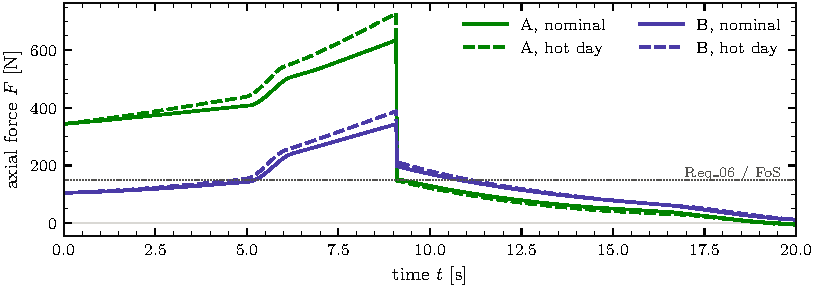
\includegraphics[width=0.8\linewidth]{figures/joint_force.pdf}}
The maximum is at burnout (highest acceleration and drag); the nose stays in compression during the
ascent ($F_\mathrm{min} \approx 0$), so the only tension case is the recovery load.

\section*{3\quad Bending moment and shear at the joint}
Normal force of the nose at incidence $\alpha$ (slender body, $C_{N\alpha} = 2$/rad) at the maximum
dynamic pressure, applied at the nose CP:
\[
V = C_{N\alpha}\,\alpha\, q_\mathrm{max}\, A_\mathrm{ref}, \qquad M_b = V\,\ell .
\]
\begin{center}\small
\begin{tabular}{@{}llrrrrrrrr@{}}
\toprule
& & & & \multicolumn{2}{c}{Limit, per degree} & \multicolumn{3}{c}{$M_b$ ultimate [N\,m]} & \\
\cmidrule(lr){5-6}\cmidrule(lr){7-9}
\multicolumn{2}{@{}l}{Case} & $q_\mathrm{max}$ [kPa] & $M$ & $M_b$ [N\,m/$^\circ$] & $V$ [N/$^\circ$] &
$\alpha = 1^\circ$ & $2^\circ$ & $5^\circ$ & $\alpha$ at Req\_12 [$^\circ$]\\
\midrule
A & nominal & 116.8 & 1.47 & 44.1 & 104 & 88 & 176 & 441 & 2.3 \\
A & hot day & 131.4 & 1.56 & 49.6 & 117 & 99 & 198 & 496 & 2.0 \\
B & nominal & 117.6 & 1.47 & 38.9 & 104 & 78 & 156 & 389 & 2.6 \\
B & hot day & 132.5 & 1.56 & 43.9 & 118 & 88 & 175 & 439 & 2.3 \\
\bottomrule
\end{tabular}
\end{center}
Req\_12 (200\,N\,m ultimate) is reached at $\alpha = 2.0^\circ$ for design A on the hot day:
the incidence that ST designs for (gusts, weathercocking) decides whether Req\_12 holds.

\section*{4\quad Wall pressure}
The highest wall pressure is at the stagnation point of the tip, $p_0 - p_\infty$ behind the normal
shock (max.\ at burnout), an upper bound for the whole shell: A 177 / 204 kPa; B 179 / 206 kPa (nominal / hot day). The pressure distribution
on the shell, $C_p(x)$, follows from the Fluent runs of REPORT-5.

\section*{5\quad Temperatures}
Laminar stagnation-point heating (Fay--Riddell) on the $r_n = 4.5$\,mm tip, turbulent
(Reynolds analogy, Eckert reference temperature) downstream; the Al 6082 tip insert (80\,mm, 60\,g)
as a lumped mass, the 1.2\,mm CFRP shell as 1D conduction with an adiabatic inner face (conservative,
bare shell without the insert). Peak values over the flight [$^\circ$C]:
\begin{center}\small
\begin{tabular}{@{}lrrrrll@{}}
\toprule
& \multicolumn{2}{c}{A} & \multicolumn{2}{c}{B} & & \\
\cmidrule(lr){2-3}\cmidrule(lr){4-5}
Location & nominal & hot day & nominal & hot day & Limit & Worst case\\
\midrule
Stagnation temperature $T_0$ (air) & 118 & 154 & 119 & 156 & -- & -- \\
Al 6082 tip insert (bond to the shell) & 58 & 81 & 53 & 75 & 120 (DP490) & ok \\
CFRP shell outer face, $x = 50$\,mm & 82 & 109 & 82 & 110 & -- & -- \\
CFRP shell inner face, $x = 50$\,mm & 77 & 103 & 77 & 104 & 67 (Req\_10) & \textbf{exceeds} \\
CFRP shell inner face, mid-length & 71 & 97 & 72 & 97 & 67 (Req\_10) & \textbf{exceeds} \\
CFRP shell inner face, shoulder & 69 & 94 & 69 & 95 & 67 (Req\_10) & \textbf{exceeds} \\
\bottomrule
\end{tabular}
\end{center}
\centerline{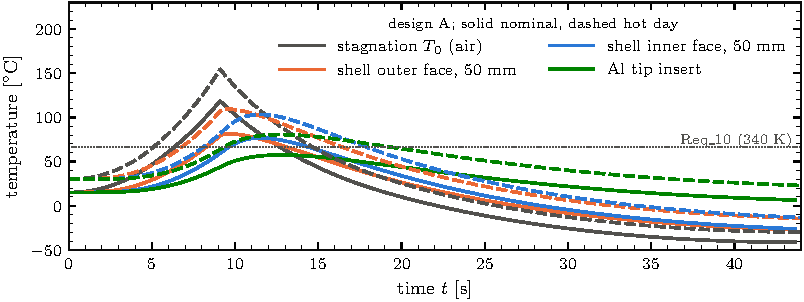
\includegraphics[width=0.8\linewidth]{figures/temperatures_A.pdf}}
Materials are the REPORT-1 assumptions (Al 6082 insert, CFRP shell 1.2\,mm, DP490 bond): to be
confirmed by ST. Fluent heat-transfer runs and an Ansys transient-thermal model of the tip will
replace these values in 2027\_C\_FD\_REPORT-5 (12.11.2026).

\section*{6\quad Open points for ST and SE}
\begin{itemize}\setlength{\itemsep}{1pt}
\item \textbf{Req\_06:} the ultimate compression exceeds 300\,N for both designs
  (A 1454\,N, B 777\,N, hot day).
  \textbf{Req\_07:} with the 3U GRV in the nose, the recovery tension of A
  (2252\,N) exceeds 2000\,N.
\item \textbf{Req\_12:} the design incidence at max $q$ must be agreed (Req\_12 is reached at
  $\approx 2^\circ$).
\item \textbf{Req\_10:} does 340\,K apply to the air in the nose or to the inner wall? The bare inner
  wall of A reaches 69--77\,$^\circ$C (nominal) against 67\,$^\circ$C.
\item \textbf{Req\_08:} the TBD values (max temperature, duration) can be filled from section 5.
\end{itemize}
\end{document}
